\chapter{ SIFT en GPU}
\spacing{1.5}
Paralelizar correctamente un algoritmo no es una tarea trivial. Después del capítulo anterior al ver todas las ventajas que tenemos en las GPU, se puede decir que son la solución a todo. Tristemente, no lo son. Existen algoritmos que, por la estructura del programa y forma de ejecutar el proceso, no se pueden paralelizar. Para saber cómo analizar si un algoritmo es paralelizable, primero se dará una definición de que es un programa paralelo:
\begin{center}
\textit{“Un programa paralelo es la especificación de dos o más procesos simultáneos que cooperan entre sí con un fin en común” \cite{concurrente}}
\end{center}
Se pueden destacar dos aspectos importantes de esta definición: el primero es la comunicación. Los procesos deben poder compartir información  para poder trabajar simultáneamente sobre un mismo problema. El segundo es la sincronización, que es simplemente como organizar a los procesos para que realicen trabajo sin que interferir al de otros procesos.\\
Entonces se debe cambiar la forma en que se hacen los programas, ahora no solo es el cómo llegar a un objetivo paso a paso, sino que además se tiene que pensar cómo muchos procesos trabajarán juntos para alcanzar un objetivo. Para lo que se debe dividir el algoritmo, los datos o los dos, para repartir el trabajo. Para paralelizar el algoritmo se analizan básicamente tres casos de paralelismo:\\\\
\begin{itemize}
	\item \textit{Funcional}: Lo que se divide es el algoritmo. Se buscan pasos en el algoritmo que no dependan de otra parte del mismo y se ejecutan simultáneamente en diferentes procesos. Requiere de sincronizar muy cuidadosamente, para que las diferentes partes del algoritmo no interfieran entre sí. 
	 \begin{figure}[H]
	 		\centering
	 			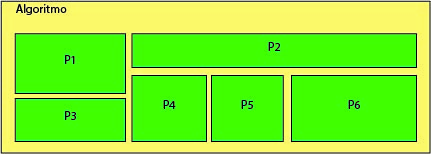
\includegraphics[height=3.5cm]{img/funcional.jpg}
	 		\caption{\textit{Funcional}:Todos los procesos son partes diferentes del algoritmo}
	 \end{figure}
	\item \textit{Dominio}: Se repartirán los datos en múltiples procesos los cuales tienen una especificación idéntica. La sincronización es sencilla en este caso, aun así hay que prestar atención ya que se podría corromper la información.
	 \begin{figure}[H]
	 		\centering
				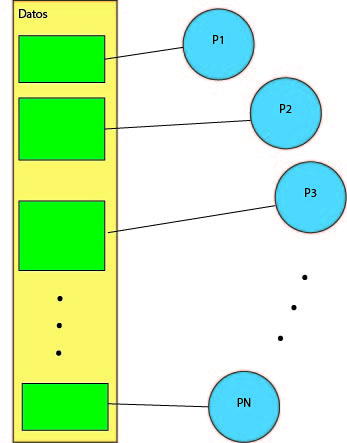
\includegraphics[height=8cm]{img/dominio.jpg}
	 		\caption{\textit{Dominio}:Todos los procesos tienen la misma especificación}
	 \end{figure}
	\item 	\textit{Actividad}: Es una combinación de los dos puntos anteriores.
\end{itemize}
Teniendo conocimiento sobre el algoritmo y las herramientas para mejorar su rendimiento por medio de la paraleización, se analizaran las partes de SIFT para de esta manera adaptarlo al modelo de programación de CUDA.
\section{Análisis de SIFT para su Paralelización en GPU}
En esta sección se describe cómo se comunicarán y sincronizarán los procesos, así como la estructura que tomará el algoritmo de SIFT para poder paralelizarlo con CUDA.\\
Primero se dividirá en 6 partes el algoritmo de SIFT, como se muestra en la figura 4-3, para facilitar la programación en diferentes kernels los cuales no serán ejecutados simultáneamente.\\
\begin{figure}[H]
			\centering
				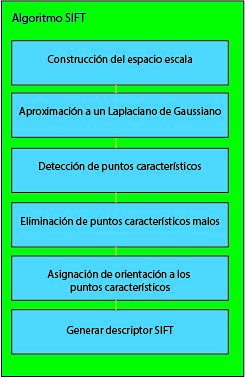
\includegraphics[height=10cm]{img/SIFTdiv.jpg}
			\caption{División del algoritmo SIFT a paralelizar}
\end{figure}
Los kernels de las diferentes partes del algoritmo tienen una estructura en común: todos tienen como entrada una o más imágenes (datos de solo lectura) y tienen como salida una imagen (o varias). Cada proceso tiene una sección de la imagen de tamaño  $N \times N$, la cual puede estar traslapada con la de algún otro proceso. Sin embargo esta área no requiere de sincronización entre procesos ya que solo se usa para obtener datos no para procesarlos. En la imagen de salida al proceso, se le será asignado un solo pixel de la imagen. Como se puede mostrar en la figura 4-4, las zonas P1 y P2 están traslapadas en la imagen de salida (como si tuviera un zoom a los pixeles) no escriben en otro que no sea su pixel.
\begin{figure}[H]
			\centering
				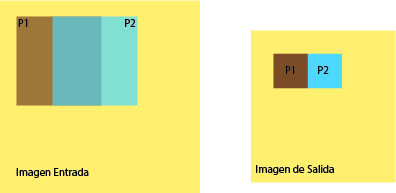
\includegraphics[height=5cm]{img/prosImg.jpg}
			\caption{Proceso general de los kenels}
\end{figure}
Los procesos que se ejecutan sobre la imagen tienen la misma especificación. Es decir que lo que estamos repartiendo entre los múltiples procesos son los datos de entrada, con lo cual estaremos en la categoría de paralelismo de \textit{dominio}.\\
Cada uno de los kernels será ejecutado múltiples veces. Este trabajo será desempeñado por el anfitrión (CPU) en forma secuencial. Esto es importante ya que cada uno de estos kernels es lanzado sin importar que el anterior terminara de ejecutarse. Si múltiples kernels son lanzados y tienen la misma especificación pero trabajan con diferentes secciones de los datos no existe problema. Pero si el anfitrión llegara a lanzar un kernel que tiene una especificación diferente a la de un banco de kernels lanzados anteriormente, y estos no han finalizado puede existir riesgo de corromper los datos. Entonces debemos de sincronizar, como se puede ver en la figura 4-5, al  dispositivo (GPU) con el anfitrión (CPU) para evitar caer en este tipo de errores.\\
\begin{figure}[H]
			\centering
				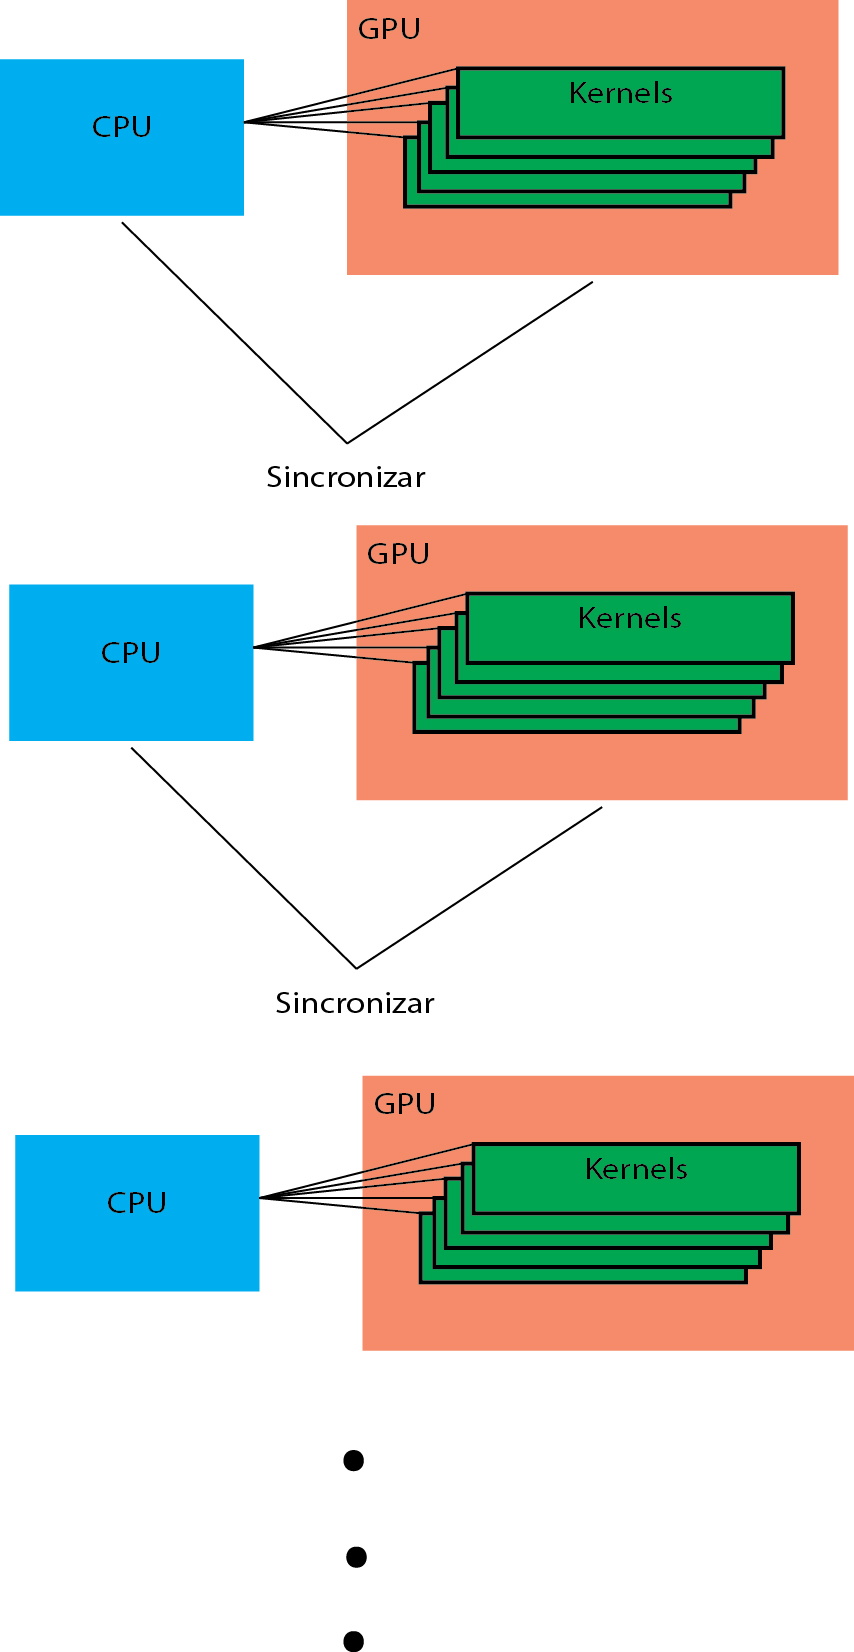
\includegraphics[height=10cm]{img/lanzamiento.jpg}
			\caption{Lanzamiento de Kernels}
\end{figure}
\section{Implementación}
Teniendo en cuenta la estructura general de la solución, se plantea como se construyó y como es el funcionamiento de cada una de las partes en las que se dividió el algoritmo de SIFT (figura 4-3), para poder adaptarlo al modelo de programación de CUDA.
\begin{figure}[H]
		\centering
		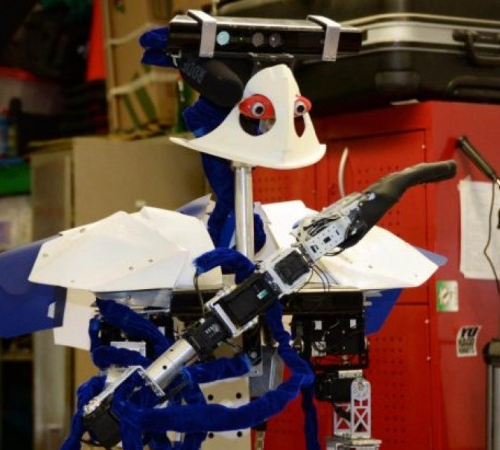
\includegraphics[height=5cm]{img/justina.jpg}
		\caption{Esta es la imagen de entrada que arrojaron como resultado las de las figuras 4-8, 4-9, y 4-11}
\end{figure}
\subsection{Construcción del espacio escala y aproximación a un Laplaciano de Gaussiana}
Para construir el espacio escala con aproximaciones a un Laplaciano de Gaussiana se usaron  diferentes filtros de diferencia de Gaussiana por cada escala, convolucionados con las imágenes de la escala.  
$$D(x,y;\sigma) = (G(x,y;k\sigma) - G(x,y;\sigma)) * I(x,y)$$ 
Para ello se obtienen los filtros Gaussianos con la ayuda de la librería OpenCV \cite{Opencv}, y se restan para así obtener los filtros que aplicados en cada octava, quedando como los de las figura 4-7.\\
 \begin{figure}[H]
 			\centering
 				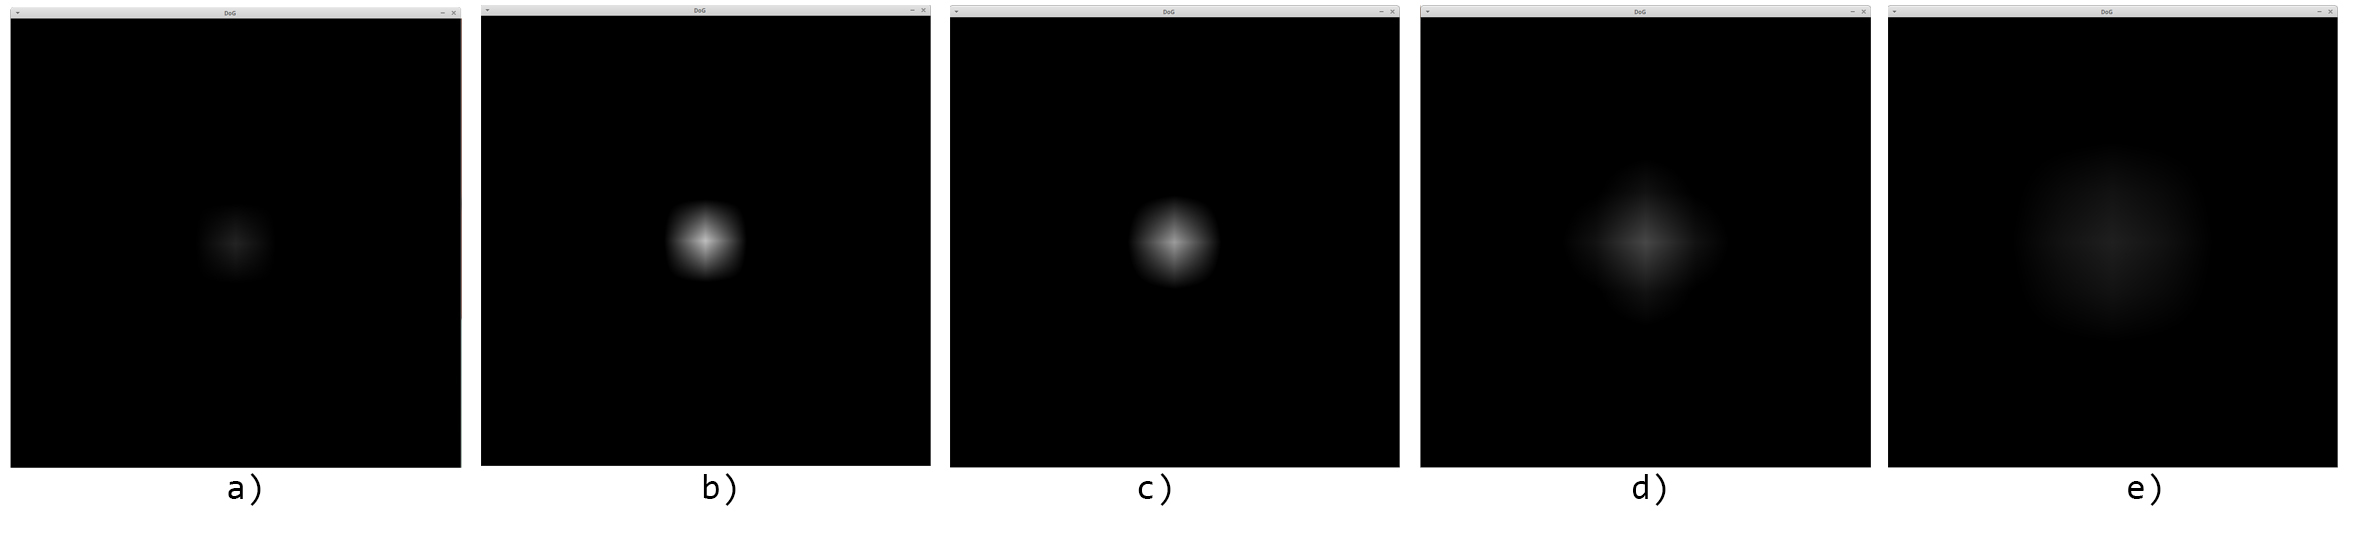
\includegraphics[width=\textwidth]{img/DoG.jpg}
 			\caption{Filtros de diferencias de gaussianas. a) $\sigma_{0}=1-\sigma_{1}=1.08$,b) $\sigma_{1}=1.08-\sigma_{2}=1.36$,c) $\sigma_{2}=1.36-\sigma_{3}=1.72$,d) $\sigma_{3}=1.72-\sigma_{4}=2.16$, e) $\sigma_{4}=2.16-\sigma_{5}=2.72$. }
 \end{figure}
También se usó OpenCV para cambiar el tamaño de las imágenes, para cada octava.
En lo que refiere a la construcción del espacio escala la parte que se paralelizo fue la convolución de una imagen y un filtro. Se puede ver como se hizo la implementación en el apéndice A.\\   
La idea es que estos kernels sean lanzados por el anfitrión. Se lanzarán tantos kernels como imágenes se necesitan para crear el espacio escala. Los kernels serán ejecutados de forma concurrente.\\
La función de cada kernel es, para cada pixel en la imagen de salida, asignar un hilo y estos se encargarán con los datos de entrada (la imagen y el filtro) de implementar la operación de convolución.\\
\begin{algorithm}[H]
\caption{Cálculo de la convolución para cada imagen del espacio escala}
 \KwData{ImgEntrada, Filtro}
 \KwResult{Img }
 Para cada pixel en ImgEntrada asigna un hilo\;
 \ForAll{hilos}
 {
	\eIf{Img.pixel es orilla}
	{
		Img.pixel=0;
	}{
		Img.pixel= ImgEntrada.zona * Filtro; 
		\tcp{Donde * es el operador para la convolución}			
	}
 }
\end{algorithm}
El resultado se ejemplifica en figura 4-8, Tendremos imágenes muy similares para cada una de las octavas. 
\begin{figure}[H]
			\centering
				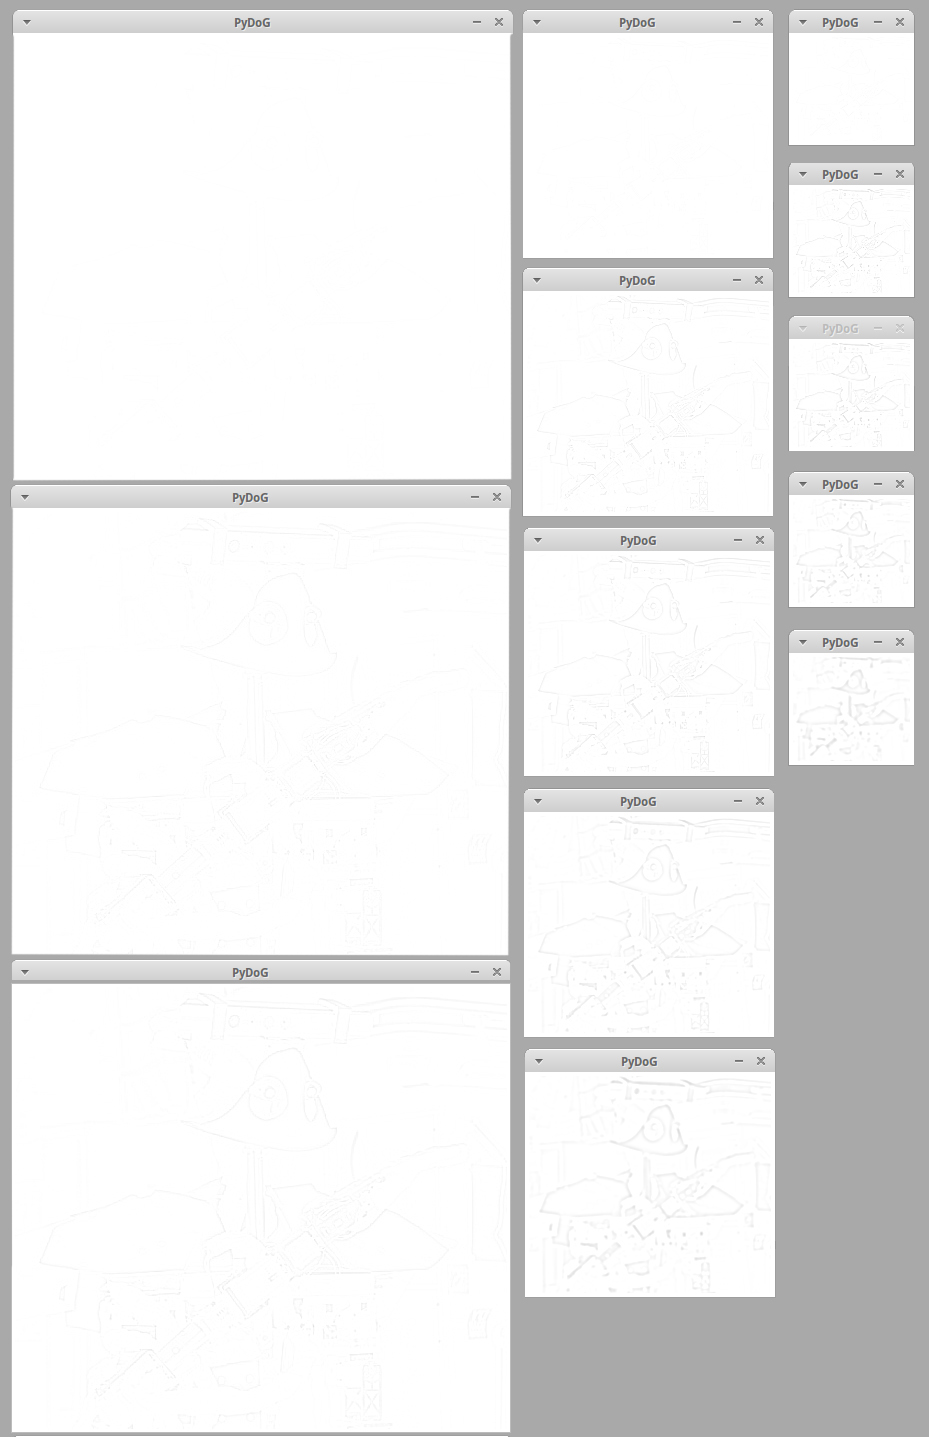
\includegraphics[height=11cm]{img/pyDoGT.jpg}
			\caption{Espacio Escala de Diferencia de Gaussiana}
\end{figure}
\subsection{Detección de puntos característicos}
En el espacio escala obtenido anteriormente se buscarán los puntos extremos. En $D(x,y,\sigma)$ se buscarán las ubicaciones máximas y mínimas. Cada punto es comparado con sus ocho vecinos en la misma imagen y con sus otros dieciocho vecinos de escala, nueve en la imagen de arriba y nueve en la imagen de abajo. Sólo se selecciona la ubicación si el pixel tiene un valor mayor o menor a todos sus vecinos.\\
\begin{algorithm}[H]
\caption{Búsqueda de puntos extremos}
 \KwData{ImgArriba, Img , ImgAbajo }
 \KwResult{ImgMascara}
 Para cada pixel en Img asigna un hilo\;
 
 \ForAll{hilos}
 {
	\eIf{Img.pixel es orilla}
	{
		ImgMascara.pixel=0\;
	}{
		\ForAll{pixel vecino a Img en ImgArriba, ImgAbajo e Img }
		{
			Compara cada pixel vecino con el pixel asignado al hilo\;
			\eIf{si todos los vecinos son menores o mayores}
			{
				ImgMascara.pixel = 1\;			
			}{
				ImgMascara.pixel = 0\;
			
			}
		
		}
		
	}
 }
\end{algorithm}
Como se puede ver en el algoritmo 2, lo que hacemos en el kernel es asignar a cada hilo un pixel de la imagen de entrada \texttt{Img} para compararla con sus vecinos y así poder determinar si es un punto extremo.\\
La imagen de salida terminará siendo una máscara binaria. Si existe un punto extremo, pondrá un pixel en blanco, y donde no, lo dejará en negro tal como se muestra en la figura 4-9; Se puede encontrar la implementación de este algoritmo en el apéndice B.
\begin{figure}[H]
			\centering
				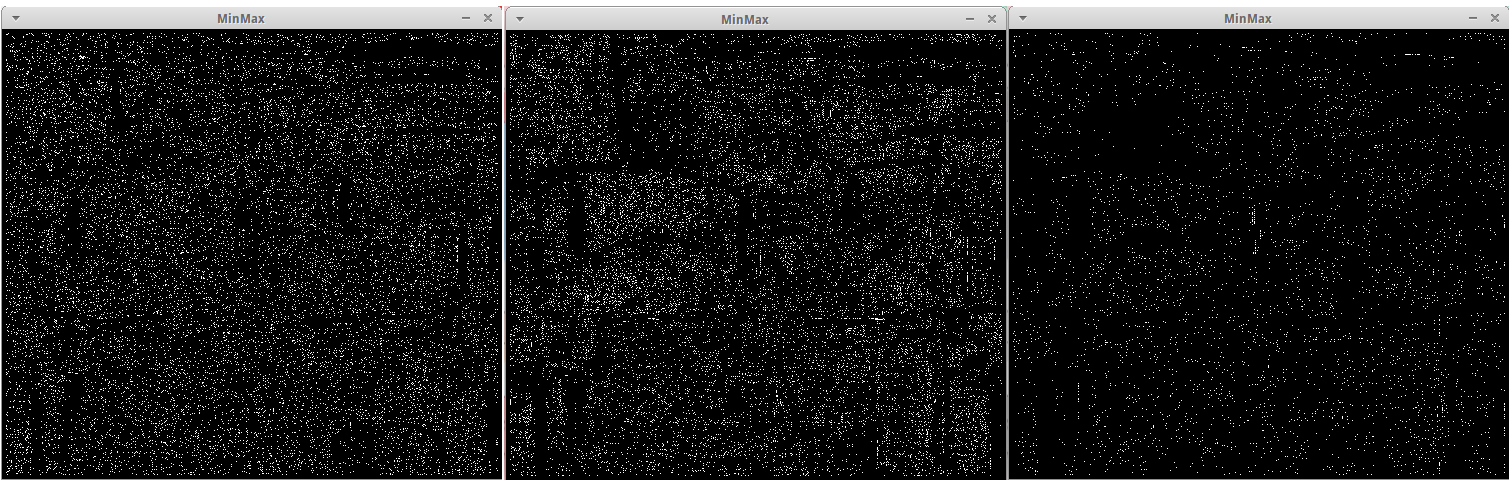
\includegraphics[width=\textwidth]{img/minmaxs.jpg}
			\caption{Mascara.  Búsqueda con las imágenes del espacio escala: a) 0,1,2 ; b) 1,2,3; c)2,3,4  }
\end{figure} 
\subsection{Eliminación de puntos característicos malos}
A continuación se filtran los puntos extremos encontrados anteriormente. Existen dos casos donde los puntos extremos anteriormente seleccionados deben de ser eliminados, el primero es donde el contraste es muy bajo y el segundo es cuando se localiza en un borde.\\
\begin{algorithm}[H]
\caption{Eliminación de puntos característicos malos}
 \KwData{Img , ImgMascara}
 \KwResult{ImgMascara}
 Para cada pixel en Img asigna un hilo\;
 \ForAll{hilos}
 {
	\If{ImgMascara.pixel es mayor que 0}
	{
		\If{Img.pixel tiene contraste bajo o está en un borde}
		{
			ImgMascara.pixel=0;
		}
	}
}
\end{algorithm}
Se obtendrá una máscara muy parecida a la de la Figura 4-10, pero esta vez se tienen muchos menos pixeles en color blanco. En el apéndice C se puede ver más detalladamente como se realizó la implementación de esta parte del algoritmo de SIFT.
\begin{figure}[H]
			\centering
				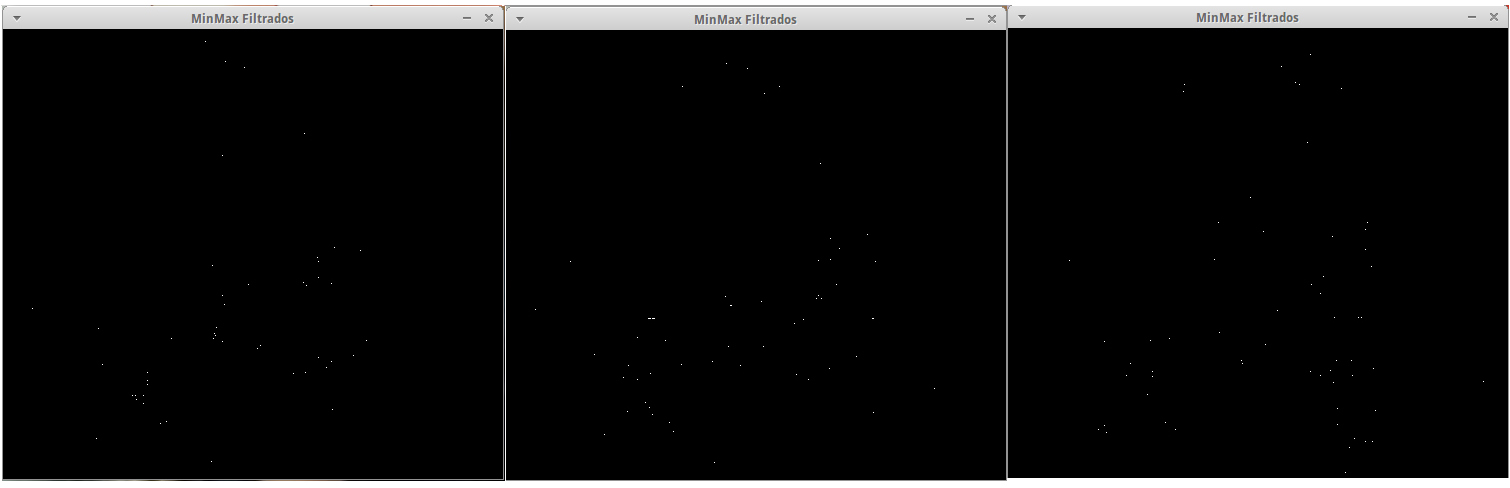
\includegraphics[width=\textwidth]{img/minmax.jpg}
			\caption{Máscara Filtrada de la búsqueda con las imágenes del espacio escala: a) 0,1,2 ; b) 1,2,3; c)2,3,4  }
\end{figure}
\subsection{Asignación de orientación a los puntos característicos}
Encontrar la orientación de cada punto característico, basado en propiedades locales de la imagen, es importante para que el descriptor sea invariante a la rotación.\\
\begin{algorithm}[H]
\caption{Cálculo de orientaciones y magnitudes en cada pixel}
 \KwData{Img}
 \KwResult{ImgMagnitud, ImgOrientacion}
 Para cada pixel en Img asigna un hilo\;
 
 \ForAll{hilos}
 {
	Calcular magnitud en Img.pixel\;
	Calcular orientación en Img.pixel\;
	ImgMagnitud.pixel= magnitud\;
	ImgOrientacion.pixel=orientación\;
	
}
\end{algorithm}
Para esta parte lo que se hizo fue dividir en dos kernels el proceso: uno para calcular las magnitudes y orientaciones de los gradientes. (Véase apéndice D)
$$m(x,y) = \sqrt{ (L(x+1,y)-L(x-1,y))^2 + (L(x,y+1)-L(x,y-1))^2 }$$		
$$\theta(x,y) =  \tan^{-1} \left(\frac{L(x,y+1)-L(x,y-1)}{L(x+1,y)-L(x-1,y)}\right)$$
Y el otro, donde se obtienen los histogramas para cada punto característico y se asigna una orientación dominante. (Véase apéndice E)\\
\begin{algorithm}[H]
\caption{Asignación de orientación respecto a su histograma}
 \KwData{Img , ImgMascara, ImgMagnitud, ImgOrientacion}
 \KwResult{PuntosCaracteristicos}
 Para cada pixel en Img asigna un hilo\;
 
 \ForAll{hilos}
 {
	\If{ImgMascara.pixel es mayor que 0}
	{
		Realizar el histograma de la zona alrededor del punto característico\;
		Encontrar cuales son los valores más altos más altos\;
		Encontrar una orientación dominante con los puntos más altos\;
		Almacenar la orientación y la ubicación de ese punto característico\; 
	
	}
}
\end{algorithm}
\begin{figure}[H]
			\centering
				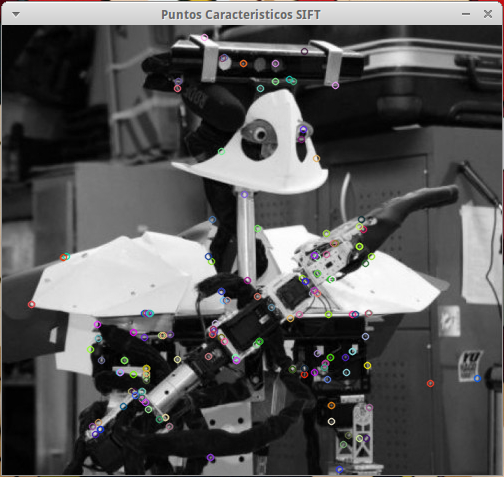
\includegraphics[height=16cm]{img/KeyPoints.png}
			\caption{Puntos característicos encontrados}
\end{figure}
